\state{Lattice specific heat}{\hfix}

\prob{}{
	From Eq.~(2.44) derive the formula for the Debye specific heat Eq.~(2.45).
}

\sol{
	Equation~(2.44) is
	\eq{
		\UD = \intoomgD \ddomg \frac{V \omg^2}{2 \pi^2 v^3} \frac{\hbar \omg}{e^{\hbar \omg / \kB T} - 1}
	}
	From Eq.~(2.43), $\CV = (\pdv*{U}{T})_V$.  As on p.~23 of the lecture notes, we multiply the right side by three since there are three acoustic branches.  So
	\eqn{CV6.a1}{
		\CV = 3 \paren{ \pdv{\UD}{T} }_V
		= 3 \intoomgD \ddomg \frac{V \omg^2}{2 \pi^2 v^3} \hbar \omg \pdv{T}(\frac{1}{e^{\hbar \omg / \kB T} - 1}).
	}
	Let $x = \hbar \omg / \kB T$.  Then
	\eq{
		\pdv{T}(\frac{1}{e^{\hbar \omg / \kB T} - 1}) = \pdv{x}{T} \pdv{x}(\frac{1}{e^x - 1})
		= \paren{ -\frac{\hbar \omg}{\kB T^2} } \paren{ -\frac{e^x}{(e^x - 1)^2} }
		= \frac{\hbar \omg}{\kB T^2} \frac{e^{\hbar \omg / \kB T}}{(e^{\hbar \omg / \kB T} - 1)^2}.
	}
	So Eq.~\refeq{CV6.a1} becomes
	\eq{
		\CV = 3 \intoomgD \ddomg \frac{V \hbar^2 \omg^4}{2 \pi^2 v^3 \kB T^2} \frac{e^{\hbar \omg / \kB T}}{(e^{\hbar \omg / \kB T} - 1)^2}
		= 3 \intoomgD \ddomg \frac{V \kB^3 T^2}{2 \pi^2 \hbar^2 v^3} \frac{x^4 e^x}{(e^x - 1)^2}.
	}
	We can write $x = \ThtD / T$, where $\ThtD = \hbar \omgD / \kB$ as on p.~23 of the lecture notes.  Then, changing our variable of integration,
	\aln{
		\CV &= 3 \intoThtDT \frac{\kB T \ddx}{\hbar} \frac{V \kB^3 T^2}{2 \pi^2 \hbar^2 v^3} \frac{x^4 e^x}{(e^x - 1)^2}
		 = 3 \intoThtDT \frac{\kB T \ddx}{\hbar} \frac{V \kB^3 T^2}{2 \pi^2 \hbar^2 v^3} \frac{x^4 e^x}{(e^x - 1)^2}
		 = 3 \frac{V \kB^4 T^3}{2 \pi^2 \hbar^3 v^3} \intoThtDT \ddx \frac{x^4 e^x}{(e^x - 1)^2} \notag \\
		 &= 3 \frac{V \omgD^3}{2 \pi^2 v^3} \kB \frac{T^3}{\ThtD^3} \intoThtDT \ddx \frac{x^4 e^x}{(e^x - 1)^2}. \label{CV6.a2}
	}
	From Eq.~(2.38),
	\eq{
		\omgD^3 = \frac{6 \pi^2 v^3 N}{V}
		\qimplies
		3 N = \frac{V \omgD^3}{2 \pi^2 v^3}.
	}
	With this, Eq.~\refeq{CV6.a2} becomes
	\eqn{CV6.a}{
		\CV = 9 N \kB \paren{ \frac{T}{\ThtD}}^3 \intoThtDT \ddx \frac{x^4 e^x}{(e^x - 1)^2},
	}
	which is Eq.~(2.45). \qed
}



\prob{}{
	Evaluate the integral at \emph{high} temperature $T \gg \ThtD$, and therefore determine the high temperature behavior of the specific heat.
}

\sol{
	When $\ThtD \ll T$, $x \ll 1$ in the integrand of Eq.~\refeq{CV6.a}, and we can Taylor expand the integrand about $x = 0$~\cite[p.~460]{Ashcroft}.  The first term of the expansion, evaluated with Mathematica, is $x^2$.  Then the specific heat is
	\eqn{CV6.b}{
		\CV \sim 9 N \kB \paren{ \frac{T}{\ThtD}}^3 \intoThtDT \ddx x^2
		= 9 N \kB \paren{ \frac{T}{\ThtD}}^3 \brac{ \frac{x^3}{3} }_{\ThtD / T}
		= \ans{ 3 N \kB. }
	}
	\vfix
}



\prob{}{
	Using the formula
	\eq{
		\intoi \ddx \frac{x^4 e^x}{(e^x - 1)^2} = \frac{4\pi^4}{15},
	}
	determine the low temperature behavior of the Debye specific heat.
}

\sol{
	Substituting the given formula into Eq.~\refeq{CV6.a} where $\ThtD / T \gg 1$ for small $T$, we find
	\eq{
		\CV \approx 9 N \kB \paren{ \frac{T}{\ThtD}}^3 \intoThtDT \ddx \frac{x^4 e^x}{(e^x - 1)^2}
		= 9 N \kB \paren{ \frac{T}{\ThtD}}^3 \frac{4\pi^4}{15}
		= \ans{ \frac{12 \pi^4}{5} N \kB \paren{ \frac{T}{\ThtD}}^3. }
	}
	\vfix
}



\prob{}{
	Sketch the heat capacity formulae from the Debye and Einstein models and compare them.
}

\sol{
	From Eqs.~\refeq{CV6.a} and \refeq{CV6.b}, the Debye specific heat goes as $(T / \ThtD)^3$ at low temperatures and as at $3 N \kB$ at high temperatures.  So the shape of the curve will be concave up for small $T / \ThtD$, and the curve will asymptote as $T / \ThtD$ from the left.

	 As stated on p.~22 of the lecture notes, the specific heat for the Einstein model is given by Eq.~(2.43),
	 \eq{
	 	\CV = 3 N \kB \paren{ \frac{\ThtE}{T} }^2 \frac{e^{\ThtE / T}}{(e^{\ThtE / T} - 1)^2}
	 }
	where $\ThtE = \hbar \omgo / \kB$, and goes as $3 e^{-\ThtE / T}$ at low temperatures and as $3 N \kB$ at high temperatures.  So the qualitative shape of the curve will be the same as for the Debye model.  However, the Debye curve will rise much more rapidly since it has an extra factor of $4 \pi^4 / 5$.  Hence, the Einstein heat capacity will always be less than the Debye heat capacity.
	
	Figure~\ref{6d} shows both heat capacity formulae.  Here, the Einstein curve is evaluated exactly with Mathematica while the Debye curve is drawn using the numerical data from Ashcroft \& Mermin~\cite[p.~461]{Ashcroft}.  As expected, both curves have the same overall shape, and the Einstein curve is below the Debye one.  The difference between the models is largest at low temperatures, where the Debye model is in better agreement with experimental data~\cite[p.~117]{Kittel}.
	
	\fig{6d}{
		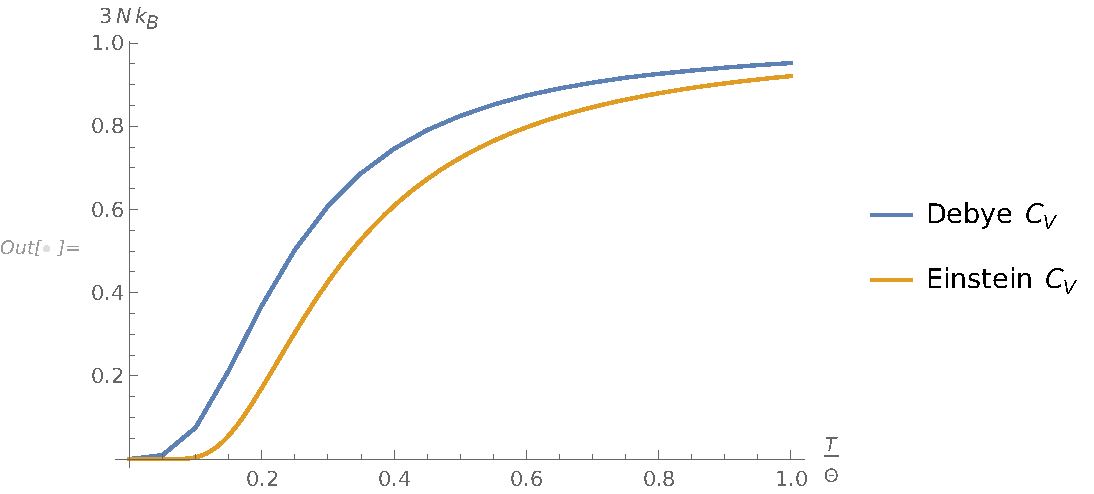
\includegraphics[width=0.75\textwidth,trim=1.5cm 0 0 0,clip]{6d}
		\caption{Comparison of the DeBye~(blue) and Einstein~(gold) heat capacity models, where $\Tht = \ThtD$ or $\ThtE$ as appropriate.}
	}
}